\documentclass[11pt, oneside]{article}

%   ==============================================================================
%   This file is part of the 3D3A MATLAB Toolkit.
%   
%   Contributing author(s), listed alphabetically by last name:
%   Rahulram Sridhar <rahulram@princeton.edu>
%   Joseph G. Tylka <josephgt@princeton.edu>
%   3D Audio and Applied Acoustics (3D3A) Laboratory
%   Princeton University, Princeton, New Jersey 08544, USA
%   
%   MIT License
%   
%   Copyright (c) 2018 Princeton University
%   
%   Permission is hereby granted, free of charge, to any person obtaining a copy
%   of this software and associated documentation files (the "Software"), to deal
%   in the Software without restriction, including without limitation the rights
%   to use, copy, modify, merge, publish, distribute, sublicense, and/or sell
%   copies of the Software, and to permit persons to whom the Software is
%   furnished to do so, subject to the following conditions:
%   
%   The above copyright notice and this permission notice shall be included in all
%   copies or substantial portions of the Software.
%   
%   THE SOFTWARE IS PROVIDED "AS IS", WITHOUT WARRANTY OF ANY KIND, EXPRESS OR
%   IMPLIED, INCLUDING BUT NOT LIMITED TO THE WARRANTIES OF MERCHANTABILITY,
%   FITNESS FOR A PARTICULAR PURPOSE AND NONINFRINGEMENT. IN NO EVENT SHALL THE
%   AUTHORS OR COPYRIGHT HOLDERS BE LIABLE FOR ANY CLAIM, DAMAGES OR OTHER
%   LIABILITY, WHETHER IN AN ACTION OF CONTRACT, TORT OR OTHERWISE, ARISING FROM,
%   OUT OF OR IN CONNECTION WITH THE SOFTWARE OR THE USE OR OTHER DEALINGS IN THE
%   SOFTWARE.
%   ==============================================================================

% Required packages
\usepackage[letterpaper, margin=1in, includeheadfoot]{geometry}
\usepackage{hyperref}
\usepackage{tabularx}

% Header and Footer
\usepackage{fancyhdr}
\pagestyle{fancy}
\renewcommand{\headrulewidth}{1pt}
\lhead{}\chead{\textsc{3D Audio and Applied Acoustics Laboratory $\cdot$ Princeton University}}\rhead{}
\lfoot{}\cfoot{\thepage}\rfoot{}

\renewcommand{\abstractname}{Summary} % Activate to modify the name of the Abstract
%\renewcommand*{\thefootnote}{\fnsymbol{footnote}} % Activate to use symbols rather than numbers for footnotes

% Additional packages
\usepackage{graphicx}
\usepackage{amssymb}
\usepackage{amsmath}
\usepackage[numbers,square,sort]{natbib}
\usepackage{tikz}
\usepackage{mathtools}

% User-defined commands
\newcommand{\citeref}[1]{Ref.~\cite{#1}}
\newcommand{\Citeref}[1]{Reference~\cite{#1}}
\newcommand{\citerefs}[1]{Refs.~\cite{#1}}
\newcommand{\Citerefs}[1]{References~\cite{#1}}
\newcommand{\figref}[1]{Fig.~\ref{#1}}
\newcommand{\Figref}[1]{Figure~\ref{#1}}
\newcommand{\figreftwo}[2]{Figs.~\ref{#1} and~\ref{#2}}
\newcommand{\eqnref}[1]{Eq.~(\ref{#1})}
\newcommand{\eqnreftwo}[2]{Eqs.~(\ref{#1}) and~(\ref{#2})}
\newcommand{\secref}[1]{Section~\ref{#1}}
\newcommand{\Secref}[1]{Section~\ref{#1}}
\newcommand{\secreftwo}[2]{Sections~\ref{#1} and~\ref{#2}}
\newcommand{\secrefthru}[2]{Sections~\ref{#1} through~\ref{#2}}
\newcommand{\tabref}[1]{Table~\ref{#1}}
\newcommand{\Tabref}[1]{Table~\ref{#1}}
\newcommand{\tabreftwo}[2]{Tables~\ref{#1} and~\ref{#2}}
\newcommand{\function}[1]{\paragraph*{\texttt{#1}}}

\begin{document}

% Title and Author block
\begin{centering}
{\Large \textbf{The 3D3A Lab's MATLAB Toolbox}}\\
\vspace{\baselineskip}
\newcolumntype{C}{>{\centering\arraybackslash}p{0.4\textwidth}} % Sets horizontal spacing between authors
\begin{tabular}{CC}
    Rahulram Sridhar & Joseph G.~Tylka \\
    \href{mailto:rahulram@princeton.edu}{rahulram@princeton.edu} & \href{mailto:josephgt@princeton.edu}{josephgt@princeton.edu}
\end{tabular}\\
\vspace{\baselineskip}
November 5\textsuperscript{th}, 2018\\
\end{centering}

% Abstract
\begin{abstract}
The 3D3A lab's MATLAB toolbox is an open-source collection MATLAB functions for spatial audio processing.
In this document, we describe the calculations performed by each of these functions.
\end{abstract}

\section{Introduction}


\section{Function Folders}

%% acoustics %%
\subsection{Acoustics}

\function{f2k} Convert temporal frequency in Hz to angular wavenumber. \\
Computes the angular wavenumber $k$ given temporal frequency $f$, such that
\begin{equation}
k = \frac{2 \pi f}{c},
\end{equation}
where $c$ is the speed of sound in air.

\function{k2f} Convert angular wavenumber to temporal frequency in Hz. \\
Computes the temporal frequency $f$ given angular wavenumber $k$, such that
\begin{equation}
f = \frac{k c}{2 \pi}.
\end{equation}

\function{f2lambda} Convert temporal frequency in Hz to wavelength. \\
Computes the wavelength $\lambda$ given temporal frequency $f$, such that
\begin{equation}
\lambda = \frac{c}{f}.
\end{equation}

\function{getSoundSpeed} Speed of sound in air. \\
Returns the speed of sound in air, given by
\begin{equation}
c = 343~\text{m/s}.
\end{equation}

\function{getPotential} Discrete Fourier transform for acoustic signals. \\
Computes the discrete acoustic potential signal $\psi[k]$ via an $N$-point FFT of an acoustic pressure signal $p[n]$, such that
\begin{equation}
\psi[k] = \frac{1}{N} \sum_{n=1}^N p[n] e^{i 2 \pi (k-1)(n-1) / N}.
\end{equation}

\function{getPressure} Inverse discrete Fourier transform for acoustic signals. \\
Computes the discrete acoustic pressure signal $p[n]$ via an $N$-point IFFT of an acoustic potential signal $\psi[k]$, such that
\begin{equation}
p[n] = \sum_{k=1}^N \psi[k] e^{-i 2 \pi (k-1)(n-1) / N}.
\end{equation}

%% ambisonics %%
\subsection{Ambisonics}

\function{ambSphericalHarmonicY} Real-valued spherical harmonic function. \\
The real-valued spherical harmonics commonly used in ambisonics are given by~\citet[section~2.2]{Zotter2009PhD}
\begin{equation}\label{eq:ambSphericalHarmonicY}
Y_l^m(\theta,\phi) = N_l^{|m|} P_l^{|m|} (\sin \theta) \times
    \begin{cases}
	\cos m \phi & \textrm{for } m \geq 0,\\
	\sin |m| \phi & \textrm{for } m < 0,
    \end{cases}
\end{equation}
where $P_l^m$ is the associated Legendre polynomial of degree $l$ and order $m$, as defined in the MATLAB \texttt{legendre} function\footnote{See:~\url{https://www.mathworks.com/help/matlab/ref/legendre.html}} by
\begin{equation}
P_l^m(x) = (-1)^m (1 - x^2)^{m/2} \frac{d^m}{dx^m} P_l(x), \quad
\textrm{with} \quad
P_l(x) = \frac{1}{2^l l!} \left[ \frac{d^l}{dx^l}(x^2 - 1)^l \right],
\end{equation}
and $N_l^m$ is a normalization term.

\function{ambNormalization} Ambisonics spherical harmonic normalization factor. \\
The orthonormal (N3D) spherical harmonics with Condon-Shortley phase\footnote{Note that including Condon-Shortley phase in the normalization term cancels it in the associated Legendre term.} is given by
\begin{equation}\label{eq:ambNormalization_N3D}
N_l^m = (-1)^m \sqrt{\frac{(2l+1)(2 - \delta_m)}{4 \pi} \frac{(l-m)!}{(l+m)!}},
\end{equation}
where $\delta_m$ is the Kronecker delta.
A commonly-used alternative is the Schmidt seminormalized (SN3D) spherical harmonic normalization convention (again with Condon-Shortley phase), given by~\citep{Nachbar2011}
\begin{equation}\label{eq:ambNormalization_SN3D}
N_l^m = (-1)^m \sqrt{\frac{2 - \delta_m}{4 \pi} \frac{(l-m)!}{(l+m)!}}.
\end{equation}

\function{ambReNormalize} Change normalization of HOA signals. \\
In general, any acoustic pressure signal $x$ may be encoded into ambisonics as a plane-wave source originating from the direction $\hat{r}$ via
\begin{equation}
a_l^m(t) = Y_l^m(\hat{r}) x(t).
\end{equation}
Letting $\tilde{Y}_l^m$ denote the spherical harmonic function with a different normalization, the corresponding ambisonics signal for that normalization is given by
\begin{equation}
\tilde{a}_l^m(t) = \tilde{Y}_l^m(\hat{r}) x(t).
\end{equation}
Consequently, $\tilde{a}_l^m$ is related to $a_l^m$ by
\begin{equation}
\tilde{a}_l^m(t) = a_l^m(t) \frac{\tilde{Y}_l^m(\hat{r})}{Y_l^m(\hat{r})} = a_l^m(t) \frac{\tilde{N}_l^{|m|}}{N_l^{|m|}}.
\end{equation}

%\function{ambNormSquared} Squared norm of the spherical harmonic function. \\
%\begin{equation}
%\| Y_l^m \|^2 = \frac{4\pi}{2l + 1} \left( N_l^0 \right)^2.
%\end{equation}

\function{getACN} Ambisonic channel number (ACN). \\
The ambisonics channel numbering (ACN) convention~\citep{Nachbar2011} is defined such that, for a spherical harmonic function of degree $l \in [0,\infty)$ and order $m \in [-l,l]$, the ACN index $n$ is given by
\begin{equation}\label{eq:getACN}
n = l (l + 1) + m.
\end{equation}

\function{getAmbOrder} Ambisonics order and degree. \\
Correspondingly, for ACN index $n$, the spherical harmonic degree and order are given by
\begin{equation}\label{eq:getAmbOrder}
\begin{aligned}
l &= \left\lfloor \sqrt{n} \right\rfloor,\\
m &= n - l (l + 1),
\end{aligned}
\end{equation}
where $\lfloor \cdot \rfloor$ denotes rounding down to the nearest integer (i.e., the ``floor'' function).

%% auditory
\subsection{Auditory}

\function{fc2erb} Equivalent rectangular bandwidth (ERB) at a center frequency. \\
\citet{GlasbergMoore1990} derived two approximations for the equivalent rectangular bandwidth, given in Hz, as a function of center frequency, given in kHz.
The first approximation is applicable at moderate sound levels and for values of $f_c$ between 0.1 and 10 kHz:
\begin{equation}\label{eq:fc2erb_1}
W_1(f_c) = 24.7(4.37 f_c + 1).
\end{equation}
The second approximation is based on the results of a number of published simultaneous masking experiments and is valid from 0.1 to 6.5 kHz:
\begin{equation}\label{eq:fc2erb_2}
W_2(f_c) = 6.23 f_c^2 + 93.39 f_c + 28.52.
\end{equation}
These two approximations are plotted in \figref{fig:fc2erb}.

\begin{figure}[tb]
    	\centering
    	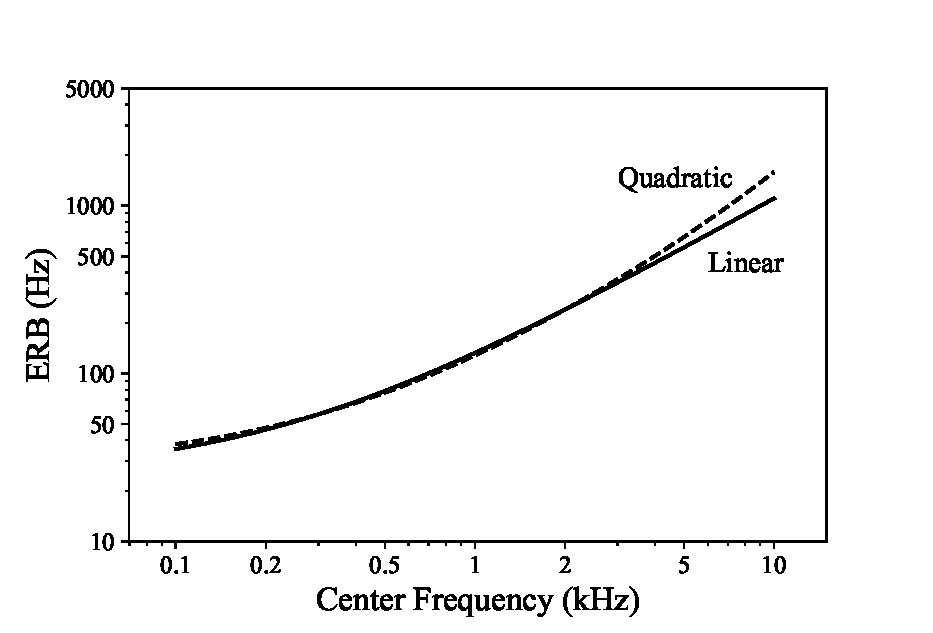
\includegraphics[width=0.55\textwidth]{figures/fc2erb.eps}
    	\caption{ERB approximations of \citet[Fig.~7]{GlasbergMoore1990}.
	The solid curve corresponds to the linear approximation, given in \eqnref{eq:fc2erb_1};
	the dashed curve corresponds to the quadratic approximation, given in \eqnref{eq:fc2erb_2}.}
	\label{fig:fc2erb}
\end{figure}

\function{getGammatoneFilters} Auditory filters that represent human critical bands. \\
This function is essentially a wrapper for the function \texttt{gammatonefir} included in the LTFAT toolbox.
The impulse responses of the gammatone filters are given by
\begin{equation}
h_\Gamma(t;f_c) = a t^3 \cos(2 \pi f_c t) e^{-2 \pi \beta t},
\end{equation}
where, for a sampling rate $F_s$, we have
\begin{equation}
\begin{aligned}
a &= \frac{2 (2 \pi \beta)^4}{3! F_s}, \\
\beta &= 1.0183 \times W_1(f_c),
\end{aligned}
\end{equation}
and $W_1(f_c)$ is the ERB at $f_c$, as given by \eqnref{eq:fc2erb_1}.

\function{getPattersonFilters} Auditory filters that represent human critical bands. \\
As given by \citet[Eq.~(5.9)]{Salomons1995PhD}, Patterson's auditory filters are given by
\begin{equation}
H_\text{P}(f;f_c) = \left( 1 + \frac{4|f-f_c|}{W_2(f_c)} \right) e^{-\frac{4|f-f_c|}{W_2(f_c)}},
\end{equation}
where $W_2(f_c)$ is the ERB at $f_c$, as given by \eqnref{eq:fc2erb_2}.

%% binaural %%
%\subsection{Binaural}

%\function{estimateITD} Estimate the interaural time difference (ITD), in seconds. \\

%%% coordinate-transforms %%%
\subsection{Coordinate Transforms}

As defined in the SOFA format~\citep{AES69-2015}, $(x,y,z) \in \mathbb{R}^3$ are the Cartesian coordinates.
\function{sofaC2sofaS} Convert SOFA cartesian coordinates to SOFA spherical coordinates. \\
The relationships between SOFA spherical coordinates, $\left(r,\theta,\phi\right)$, and SOFA cartesian coordinates, $\left(x,y,z\right)$, are given by
\begin{align}
r &= \sqrt{x^2 + y^2 + z^2}, \\
\theta &= \arctan \left(\frac{y}{x}\right) \mod 360, \\
\phi &= \arcsin \left(\frac{z}{\sqrt{x^2 + y^2 + z^2}}\right),
\end{align}
where mod denotes the modulo operation, and the ranges, in degrees, of the $\arctan$ and $\arcsin$ functions are $\left[-180,180\right]$ and $\left[-90,90\right]$, respectively.
The resulting $r$, $\theta$, and $\phi$ have the following ranges: $r \in (0,\infty)$, $\phi \in \left[-90,90\right]$, and $\theta \in \left[0,360\right)$.
Elevation, $\phi$, and azimuth, $\theta$, are specified in degrees.

\function{sofaS2sofaC} Convert SOFA spherical coordinates to SOFA cartesian coordinates. \\
The relationships between SOFA cartesian coordinates, $\left(x,y,z\right)$, and SOFA spherical coordinates, $\left(r,\theta,\phi\right)$, are given by
\begin{align}
x &= r \cos \phi \cos \theta, \\
y &= r \cos \phi \sin \theta, \\
z &= r \sin \phi,
\end{align}
where $r \in (0,\infty)$.
Elevation, $\phi \in \left[-90,90\right]$, and azimuth, $\theta \in \left[0,360\right)$, are specified in degrees.

\function{sofaC2cipicI} Convert SOFA cartesian coordinates to CIPIC interaural coordinates. \\
The relationships between CIPIC interaural coordinates, $\left(r,\vartheta,\varphi\right)$, and SOFA cartesian coordinates, $\left(x,y,z\right)$, are given by
\begin{align}
r &= \sqrt{x^2 + y^2 + z^2}, \\
\vartheta &= \arcsin \left(\frac{-y}{\sqrt{x^2 + y^2 + z^2}}\right), \\
\varphi &= 
\begin{cases*}
\varphi' - 360, & $\forall\,x \geq 0$ and $z < 0$, \\
\varphi', & otherwise,
\end{cases*}
\end{align}
where
\begin{equation}
\varphi' =  \arctan \left(\frac{z}{x}\right) \mod 360,
\end{equation}
with mod denoting the modulo operation, and the ranges, in degrees, of the $\arctan$ and $\arcsin$ functions being $\left[-180,180\right]$ and $\left[-90,90\right]$, respectively.
The resulting $r$, $\vartheta$, and $\varphi$ have the following ranges: $r \in (0,\infty)$, $\varphi \in \left[-90,270\right)$, and $\vartheta \in \left[-90,90\right]$.
Elevation, $\varphi$, and azimuth, $\vartheta$, are specified in degrees.
The conventions for the CIPIC interaural coordinates are specified by~\citet{Algazi2001}.

\function{cipicI2sofaC} Convert CIPIC interaural coordinates to SOFA cartesian coordinates. \\
The relationships between SOFA cartesian coordinates, $\left(x,y,z\right)$, and CIPIC interaural coordinates, $\left(r,\vartheta,\varphi\right)$, are given by
\begin{align}
x &= r \cos \vartheta \cos \varphi, \\
y &= -r \sin \vartheta, \\
z &= r \cos \vartheta \sin \varphi,
\end{align}
where $r \in (0,\infty)$.
Elevation, $\varphi \in \left[-90,270\right)$, and azimuth, $\vartheta \in \left[-90,90\right]$, are specified in degrees.
The conventions for the CIPIC interaural coordinates are specified by~\citet{Algazi2001}.

%% dsp %%
\subsection{DSP}

\function{clip} Limit the range of values of a signal. \\
\begin{equation}
y =
\begin{cases}
y_\text{min}, & \text{for}~x < x_\text{min}, \\
x, & \text{for}~x \in [x_\text{min}, x_\text{max}], \\
y_\text{max}, & \text{for}~x > x_\text{max}.
\end{cases}
\end{equation}

\function{computeBandAvg} Averages of a function in specified frequency bands. \\
For fractional-octave bands, a \texttt{logmean} (see \eqnref{eq:logmean}) is taken over a specified bandwidth of $B$ octaves, from $f_c / 2^{\frac{B}{2}}$ to $f_c \times 2^{\frac{B}{2}}$.
Alternatively, for ERB-spaced auditory bands,
\begin{equation}
\overline{X}[f_c] = \frac{\displaystyle \sum_{k=0}^{K-1} \left| H_\Gamma[k;f_c] \right| X[k]}{\displaystyle \sum_{k=0}^{K-1} \left| H_\Gamma[k;f_c] \right|}
\end{equation}

\function{fractionalOctaveSmooth} Fractional-octave smoothing of transfer functions. \\
Used to perform fractional-octave smoothing of a transfer function.
\begin{equation}\label{eq:fractionalOctaveSmooth}
H_\text{s}[k] = \sum_{k' = 0}^{N - 1} M[k, k'] H[k'].
\end{equation}

\function{computeSmoothingMatrix} Fractional-octave smoothing matrix. \\
Used for computing the smoothing matrix $M$.
Currently, the methods of \citet{HatziantoniouMourjopoulos2000} and \citet{Tylka2017} have been implemented.

\function{fftConv} Convolve two causal signals in the frequency domain. \\

\function{getForwardSTFT} Spectrogram using short-time Fourier transform (STFT). \\

\function{getInverseSTFT} Inverse short-time Fourier transform (STFT). \\

\function{getTimeVec} Vector of linearly-spaced time values. \\
Given a vector length $N$ and sampling rate $F_s$, the vector of time values $t[n]$ is given by
\begin{equation}
t[n] = \frac{n}{F_s}, \quad\quad \text{for} ~ n \in [0, N-1].
\end{equation}

\function{getFreqVec} Vector of linearly-spaced frequencies. \\
Given a vector length $K$ and sampling rate $F_s$, the vector of frequencies $f[k]$ is given by
\begin{equation}
f[k] = \frac{k F_s}{K}, \quad\quad \text{for} ~ k \in [0, K-1].
\end{equation}

\function{getMagSpec} Compute magnitude spectrum. \\

\function{getMagSpecdB} Compute magnitude spectrum in dB. \\

\function{thresholdIRs} Find the onset(s) of input IR(s) using thresholding. \\

%\function{inverseFilter} Compute an inverse filter with optional regularization. \\
%\begin{equation}\label{eq:inverseFilter}
%G(f) = \frac{H^\ast(f)}{H^\ast(f) H(f) + \beta(f)},
%\end{equation}

%\begin{figure}
%\centering
%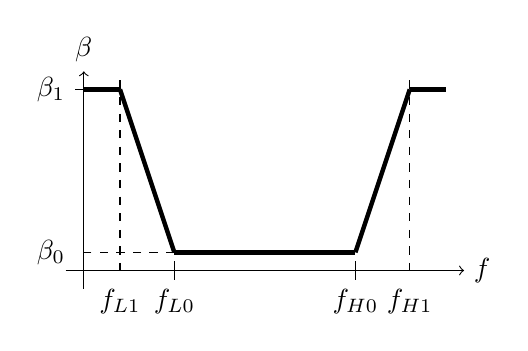
\begin{tikzpicture}[scale=2.3]
% Parameters
\def\betaone{1}; \def\betazero{0.1};
\def\fzero{0}; \def\fNyq{2};
\def\fLone{0.2}; \def\fLzero{0.5};
\def\fHzero{1.5}; \def\fHone{1.8};

% Axes
\draw[->] (\fzero-0.1,0) -- (\fNyq+0.1,0) node[right]{$f$};
\draw[->] (\fzero,-0.1) -- (\fzero,\betaone+0.1) node[above]{$\beta$};

% Tick labels
\draw (\fzero+0.05,\betaone) -- (\fzero-0.05,\betaone) node[left]{$\beta_1$};
\draw[dashed] (\fLzero,\betazero) -- (\fzero-0.05,\betazero) node[left]{$\beta_0$};
\draw[dashed] (\fLone,\betaone+0.05) -- (\fLone,-0.05) node[below]{$f_{L1}$};
\draw (\fLzero,0.05) -- (\fLzero,-0.05) node[below]{$f_{L0}$};
\draw (\fHzero,0.05) -- (\fHzero,-0.05) node[below]{$f_{H0}$};
\draw[dashed] (\fHone,\betaone+0.05) -- (\fHone,-0.05) node[below]{$f_{H1}$};

% Plot
\draw[ultra thick] (\fzero,\betaone) -- (\fLone,\betaone);
\draw[ultra thick] (\fLone,\betaone) -- (\fLzero,\betazero);
\draw[ultra thick] (\fLzero,\betazero) -- (\fHzero,\betazero);
\draw[ultra thick] (\fHzero,\betazero) -- (\fHone,\betaone);
\draw[ultra thick] (\fHone,\betaone) -- (\fNyq,\betaone);
\end{tikzpicture}
%\caption{Frequency-dependent regularization function of the inverse filters for HRTF equalization.}\label{fig:beta}
%\end{figure}

%% general %%
\subsection{General}

\function{findNearest} Find the row of a matrix nearest to a given row vector. \\

\function{loadGridFile} Load a spherical grid from a MAT file. \\

%% general data processing %%
\subsection{General Data Processing}

\function{getYRep} Compute a spherical harmonic representation of input data. \\

\function{makePosMat} Construct a matrix of position coordinate groups. \\

\function{spatialSort} Sort spatial data based on corresponding position data. \\

%% math %%
\subsection{Math}

\function{computeY} Compute spherical harmonics of specific degrees. \\

\function{computeYMat} Compute spherical harmonics of all degrees up to a specified maximum degree. \\

\function{logAvg} Log-weighted average of a function.
See also, \texttt{logmean}. \\

\function{logSTD} Log-weighted standard deviation.
See also, \texttt{logvar}. \\

\function{logmean} Log-scale average of a function. \\
Consider a discrete spectrum $X[k]$ for $k \in [0, K-1]$, where the frequency index, $k$, is proportional to the frequency in Hz, given by $k F_s/K$, and $F_s$ is the sampling rate.
We define the logarithmically-weighted average, $\overline{X}$, over the frequency index range $[K_1, K_2]$, as a weighted average
\begin{equation}\label{eq:logmean}
\overline{X} = \frac{\displaystyle \sum_{k=K_1}^{K_2} \frac{1}{k} \cdot X[k]}{\displaystyle \sum_{k=K_1}^{K_2} \frac{1}{k}}.
\end{equation}

\function{logvar} Log-scale variance of a function. \\
Similarly, we define the logarithmically-weighted variance $\sigma_X^2$ by
\begin{equation}\label{eq:logvar}
\sigma_X^2 = \frac{\displaystyle \sum_{k=K_1}^{K_2} \frac{1}{k} \left( X[k] - \overline{X} \right)^2}{\displaystyle \sum_{k=K_1}^{K_2} \frac{1}{k}}.
\end{equation}

\function{normalizeVector} Normalize vectors to unit magnitude. \\
Returns the unit vector $\hat{r}$ given a vector $\vec{r}$, such that
\begin{equation}
\hat{r} = \frac{\vec{r}}{\|\vec{r}\|} = \frac{\vec{r}}{\sqrt{\langle \vec{r}, \vec{r} \rangle}},
\end{equation}
where $\langle \cdot, \cdot \rangle$ denotes the inner product.

\function{sphericalBesselJ} Spherical Bessel function. \\
Returns the spherical Bessel function of order $n$, given by
\begin{equation}
j_n(x) =
\begin{cases}
\displaystyle \sqrt{\frac{\pi}{2 x}} J_{n+0.5}(x), & x \geq 0 \\
\displaystyle -\sqrt{\frac{\pi}{2 x}} J_{n+0.5}(x), & x < 0
\end{cases}
\end{equation}
where $J_n$ is the Bessel function of order $n$.

\function{sphericalHankelH} Spherical Hankel function. \\
Returns the spherical Hankel function of the $k^\text{th}$ kind and of order $n$, given by
\begin{equation}
h^{(k)}_n(x) =
\begin{cases}
\displaystyle \sqrt{\frac{\pi}{2 x}} H^{(k)}_{n+0.5}(x), & x \geq 0, \\
\displaystyle -\sqrt{\frac{\pi}{2 x}} H^{(k)}_{n+0.5}(x), & x < 0,
\end{cases}
\end{equation}
where $H^{(k)}_n$ is the Hankel function of the $k^\text{th}$ kind and of order $n$.

%% metrics %%
\subsection{Metrics}

\function{computeNCC} Compute maximum of the normalized cross-correlation. \\

\function{computeREE} Compute relative energy error. \\

\function{computeRMSE} Compute root-mean-squared error. \\

\function{computeSD} Compute spectral distortion. \\

\function{computeSDR} Compute signal-to-distortion ratio. \\

\function{boren2015\_Epk} Boren's peak and notch errors. \\
The peak and notch errors ($E_{\text{pk}}, E_\text{n}$) were defined by~\citet{Boren2015}
and essentially quantify the average peak (or notch) height (depth) in a frequency response over a certain frequency range.
First, the difference (in dB) is computed between finely- and coarsely-smoothed versions of the the normalized transfer function $F(f) = G(f)/G_0(f)$, i.e.,
\begin{equation}
D(f) = 20 \log_{10} \left( \frac{ \mathcal{S}\left( |F(f)|; 1/48 \right) }{ \mathcal{S}\left( |F(f)|; 1 \right) } \right),
\end{equation}
where $\mathcal{S}(F; B)$ denotes fractional-octave smoothing\footnote{In this function, we used the method described by~\citet{Tylka2017}.} applied to the spectrum $F$ with smoothing bandwidth $B$ octaves.
The peak- and notch-finding algorithms described by~\citeauthor{Boren2015}~are then applied to find the frequencies $f_1^\uparrow, f_2^\uparrow, \dots f_{N_\text{pk}}^\uparrow$ of all $N_\text{pk}$ spectral peaks and $f_1^\downarrow, f_2^\downarrow, \dots f_{N_\text{n}}^\downarrow$  of all $N_\text{n}$ spectral notches in the range $f \in [f_\text{L}, f_\text{U}]$.
The peak and notch errors are then given by~\citep[Eq.~(1)]{Boren2015}
\begin{equation}
E_\text{pk} = \frac{\sum_{j = 1}^{N_\text{pk}} D(f_j^\uparrow)}{3 \log_2 (f_\text{U}/f_\text{L})}
\quad\quad\text{and}\quad\quad
E_\text{n} = \frac{\sum_{j = 1}^{N_\text{n}} (-D(f_j^\downarrow))}{3 \log_2 (f_\text{U}/f_\text{L})},
\end{equation}
respectively. Note that, since $D$ is given in dB, the negative sign in the second equation typically ensures that both metrics are positive-valued.

\function{computeDirectionalError} Directional error between two vectors. \\
Computes a directional error between two vectors, $\vec{r}_1$ and $\vec{r}_2$, such that
\begin{equation}
\epsilon = \cos^{-1} \left( \hat{r}_1 \cdot \hat{r}_2 \right).
\end{equation}
Alternatively,
\begin{equation}
\epsilon = \sqrt{ \left\langle \left( \hat{r}_1 - \hat{r}_2 \right), \left( \hat{r}_1 - \hat{r}_2 \right) \right\rangle }.
\end{equation}

\function{estimateAudibleEnergy} Average energy in auditory critical bands. \\
We define the \textit{mean audible energy} (MAE) of a signal as its average energy in critical bands, i.e.,
\begin{equation}\label{eq:estimateAudibleEnergy}
\text{MAE} = \frac{1}{N_b} \sum_{c = 1}^{N_b} \int_{-\infty}^\infty |\Gamma(f;f_c)| |X(f)|^2 df,
\end{equation}
where $X$ is the Fourier transform of some signal and $\Gamma(f;f_c)$ is the transfer function of a gammatone filter\footnote{In this work, we used the gammatone filters implemented in the large time-frequency analysis toolbox (LTFAT) for MATLAB:~\url{http://ltfat.sourceforge.net/}} with center frequency $f_c$ for $c \in [1, N_b]$, for a set of ERB-spaced (equivalent rectangular bandwidth) center frequencies~\citep{GlasbergMoore1990} spanning the range $f \in [20~\text{Hz}, 20~\text{kHz}]$.

\function{gerzon1992} Gerzon's localization vectors. \\
Implements the velocity and energy vectors of \citet{Gerzon1992}.

\function{kates1984} Kates' central spectrum coloration model. \\
Implements the central spectrum coloration model of \citet{Kates1984}.

\function{merimaa2005} Merimaa's intensity vector and diffuseness parameter. \\
Implements the intensity vector and diffuseness parameter, computed from first-order ambisonics signals, as given by \citet{MerimaaPulkki2005}.

\function{pulkki1999\_CLL} Pulkki's composite loudness level model. \\
Implements the composite loudness level model of \citet{Pulkki1999}.

\function{scharer2009} Scharer's spectral errors in auditory bands. \\
The auditory band spectral error (ABSE), adapted from~\citet[Eq.~(9)]{ScharerLindau2009}, is given by
\begin{equation}\label{eq:scharer2009}
\eta(f_c) = 10 \log_{10} \left( \frac{\displaystyle \int_{-\infty}^\infty |H_\Gamma(f;f_c)| |G(f)|^2 df}{\displaystyle \int_{-\infty}^\infty |H_\Gamma(f;f_c)| |G_0(f)|^2 df} \right),
\end{equation}
where $G$ and $G_0$ are the transfer functions of the input and reference signals, respectively.

\function{stitt2016} Stitt's precedence-effect-based energy vector. \\
Implements the precedence-effect-based energy vector model of \citet{Stitt2016}.

\function{tylka2017} Tylka's precedence-effect localization model for ambisonics. \\
Implements the ambisonics localization vector model of \citet{TylkaChoueiri2017a}.

\function{wittek2007} Wittek's spectral alterations coloration model. \\
\citet{Wittek2007} adapted the internal spectrum (IS) defined by~\citet[chapter~5]{Salomons1995PhD} in order to define so-called \textit{spectral alterations}.
These spectral alterations are computed as the difference (in dB) between the internal spectra for the test and reference samples, given by
\begin{equation}
\text{IS}(f_c) = \text{IS}(f_c) - \text{IS}_0(f_c).
\end{equation}
According to~\citet[section~3.2.5]{Wittek2007}, the IS for each sample is given as the average of the binaural power spectra, i.e.,
\begin{equation}
\text{IS}(f_c) = 10 \log_{10} \left( \frac{P^\text{L}(f_c) + P^\text{R}(f_c)}{2} \right).
\end{equation}
Here, $P_{\text{T},\text{R}}^{\text{L},\text{R}}$ are the binaural power spectra after critical-band filtering, given by~\citep[Eq.~(5.12)]{Salomons1995PhD}
\begin{equation}
P^{\text{L},\text{R}}(f_c) = \frac{\displaystyle \int_{-\infty}^\infty |H_\text{P}(f;f_c)| |B^{\text{L},\text{R}}(f)|^2 df}{\displaystyle \int_{-\infty}^\infty |H_\text{P}(f;f_c)| df},
\end{equation}
where $H_\text{P}(f;f_c)$ are Patterson's auditory filters as specified by~\citet[Eq.~(5.9)]{Salomons1995PhD}
and $B^{\text{L},\text{R}}$ are the binaural transfer functions.

%% amt-wrappers %%
\subsubsection{Wrappers for Functions in the Auditory Modeling Toolbox}

The following functions require the Auditory Modeling Toolbox and its dependencies.

\function{wierstorf2013\_getLookupTable} ITD to azimuth lookup table. \\

\function{wrap\_may2011} Wrapper for may2011 from the Auditory Modeling Toolbox. \\

\function{wrap\_wierstorf2013} Wierstorf's azimuthal binaural localization model.

%% point-cloud-processing
\subsection{Point Cloud Processing}

\function{clusterPC} Cluster points in a point cloud based on distance of points from origin. \\

\function{declusterPC} Generate a single point cloud from a cluster of point clouds that have been clustered based on distance of points from origin. \\

\function{downsamplePC} Downsample a point cloud to approximately contain a specified number of points. \\

\function{getClusterPCYRep} Compute a spherical harmonic representation of a set of point clouds that have been clustered based on distance of points from origin. \\

\function{getPCYRep} Compute spherical harmonic representation of a point cloud assuming the point cloud is a star-shaped object (i.e. a single-valued function on a sphere). \\

%% stimuli %%
\subsection{Stimuli}

\function{exponentialSineSweep} Generate an exponential sine sweep (ESS). \\
Implements the exponential sine sweep (ESS) of \citet{Farina2000} and the phase-controlled ESS of \citet{VetterdiRosario2011}.
The conventional ESS discrete-time signal is given by~\cite{Farina2000}
\begin{equation}
x[k] = \sin \left\{ \frac{\omega_1\,N}{\ln\left(\omega_2/\omega_1\right)} \cdot \left[\left(\frac{\omega_2}{\omega_1}\right)^{\frac{k}{N}}-1\right] \right\}
\end{equation}
for $k \in[0,N-1]$, where $N = F_s T$ is the total number of samples of the signal, $T$ is the sweep duration in seconds, $F_s$ is the sampling rate in samples/second, and $\omega_1$ and $\omega_2$ are the initial and final frequencies of the sweep, respectively, in rad/sample. Note that $\omega$ represents the \textit{normalized} frequency, such that the frequency in Hz is given by $\omega F_s/2 \pi$.

The so-called ``phase-controlled'' ESS requires that the phase of the sinusoid both starts and ends at an integer multiple of $2 \pi$, yielding an amplitude of zero at the start and end of the sweep~\cite{VetterdiRosario2011}. This is accomplished by constraining the final frequency to be an integer number of octaves $P$ above the initial frequency, such that $\omega_2/\omega_1=2^P$, and by allowing some flexibility in the sweep duration. The sweep $x_{pc}[n]$ is defined by~\cite{VetterdiRosario2011}
\begin{equation}
x_{pc}[k] = \sin \left[ \frac{ \omega_1 L}{\ln \left( 2^P \right)} \cdot \left( 2^P \right)^{\frac{k}{N}} \right]
\end{equation}
for $k \in[0,N-1]$, where $L$ is the so-called ``ideal'' sweep length in samples and $N$ is the actual sweep length, equal to $L$ rounded to the nearest integer. The ideal sweep length $L$ is found based on an approximate sweep duration $T$ (in seconds) such that 
\begin{equation}
\frac{\omega_1 L}{\ln \left( 2^P \right)} = 2 \pi \cdot \textrm{Round} \left[ \frac{\omega_1 T F_s}{2 \pi \ln \left( 2^P \right)} \right].
\end{equation}
For a phase-controlled sweep that terminates at the Nyquist frequency, we will refer to the sweep by its nominal initial frequency $\omega_1 F_s/2 \pi$ and duration $T$. $L$ is then computed as shown above, and the actual $\omega_1$ is found by rounding the nominal number of octaves.

\function{warpedSineSweep} Generate a warped sine sweep. \\
Implements the warped sine sweep of \citet{OchiaiKaneda2013}.

% References
\bibliographystyle{unsrtnat}
\bibliography{refs}

\end{document}